\chapter{web自动化}
\section{selenium介绍}
\href{https://www.selenium.dev/}{Selenium}是一个开源的测试工具，用于测试Web应用程序。
Selenium是一个用于测试Web应用程序的开源工具。它提供了一种简单的API，可以通过编程方式控制浏览器的行为，从而实现自动化测试。

\subsection{组成部分}
\begin{enumerate}[label=\arabic*)]
    \item Selenium WebDriver：这是 Selenium 的核心组件，用于直接与浏览器进行交互。WebDriver 提供了丰富的 API，允许开发者通过代码控制浏览器的行为，如打开网页、点击按钮、填写表单等。
    \item Selenium IDE：这是一个浏览器插件，主要用于录制和回放用户的操作。Selenium IDE 适合初学者快速创建简单的测试脚本，但它不支持复杂的逻辑和条件判断。
    \item Selenium Grid：这是一个用于并行执行测试的工具。通过 Selenium Grid，你可以在多个浏览器和操作系统上同时运行测试，从而加快测试速度并提高测试覆盖率。
\end{enumerate}

\subsection{Selenium WebDriver}
Selenium WebDriver 是 Selenium 的核心组件，它提供了与浏览器交互的 API，允许开发者通过编程语言控制浏览器并执行各种操作。

在 Selenium 4 中，引入了 \codeinline{Service} 对象来设置驱动程序路径，这种方式更加灵活，且符合 Selenium 4 的设计规范。

\section{selenium安装}
\begin{enumerate}[label=\arabic*)]
    \item pip安装selenium
\begin{lstlisting}[style=demostyle,numbers=none]
$> pip install selenium
$> pip show selenium
Name: selenium
Version: 4.38.0
Summary: Official Python bindings for Selenium WebDriver
Home-page: https://www.selenium.dev
Author:
Author-email:
License: Apache-2.0
Location: d:\application\miniconda\envs\pyauto\lib\site-packages
Requires: certifi, trio, trio-websocket, typing_extensions, urllib3, websocket-client
Required-by:
\end{lstlisting}

    \item 下载selenium驱动程序
 
    在selenium4.6以前的版本中，selenium需要下载对应的浏览器的驱动程序，才能进行自动化测试。
    \begin{table}
        \centering
        \begin{tabular}{|c|c|c|}
            \hline
            浏览器 & 驱动程序 & 下载地址 \\
            \hline
            Chrome & ChromeDriver & \href{https://sites.google.com/chromium.org/driver/}{点击下载} \\
            \hline
            Edge & EdgeDriver & \href{https://developer.microsoft.com/en-us/microsoft-edge/tools/webdriver/}{点击下载} \\
            \hline
            Firefox & GeckoDriver & \href{https://github.com/mozilla/geckodriver/releases}{点击下载} \\
            \hline
            Safari & SafariDriver & \href{https://webkit.org/blog/6900/webdriver-support-in-safari-10/}{点击下载} \\
            \hline
        \end{tabular}
    \end{table}
\end{enumerate}

\section{启动浏览器}
\begin{enumerate}[label=\arabic*)]
    \item selenium4.6以前的版本
\begin{lstlisting}[style=demostyle,numbers=none]
from selenium import webdriver

# 使用 Chrome 浏览器
driver = webdriver.Chrome(executable_path='/path/to/chromedriver')

# 或者使用 Firefox 浏览器
# driver = webdriver.Firefox(executable_path='/path/to/geckodriver')

# 或者使用 Edge 浏览器
# driver = webdriver.Edge(executable_path='/path/to/msedgedriver')
\end{lstlisting}

    \item selenium4.6及以后版本

    在 Selenium 4 中，不再直接在 webdriver.Chrome 中设置驱动程序路径，而是通过引入 Service 对象来设置。这样可以避免弃用警告，并确保驱动程序的正确加载。例如：
\begin{lstlisting}[style=demostyle,numbers=none]
from selenium import webdriver
driver = webdriver.Chrome() # 如果使用其他浏览器，如 Firefox，需要相应修改

# 访问网址
driver.get(f"https://www.baidu.com/")

# 保持浏览器不退出
s = input("输入回车退出")
\end{lstlisting}
\begin{figure}[htpb]
    \centering
    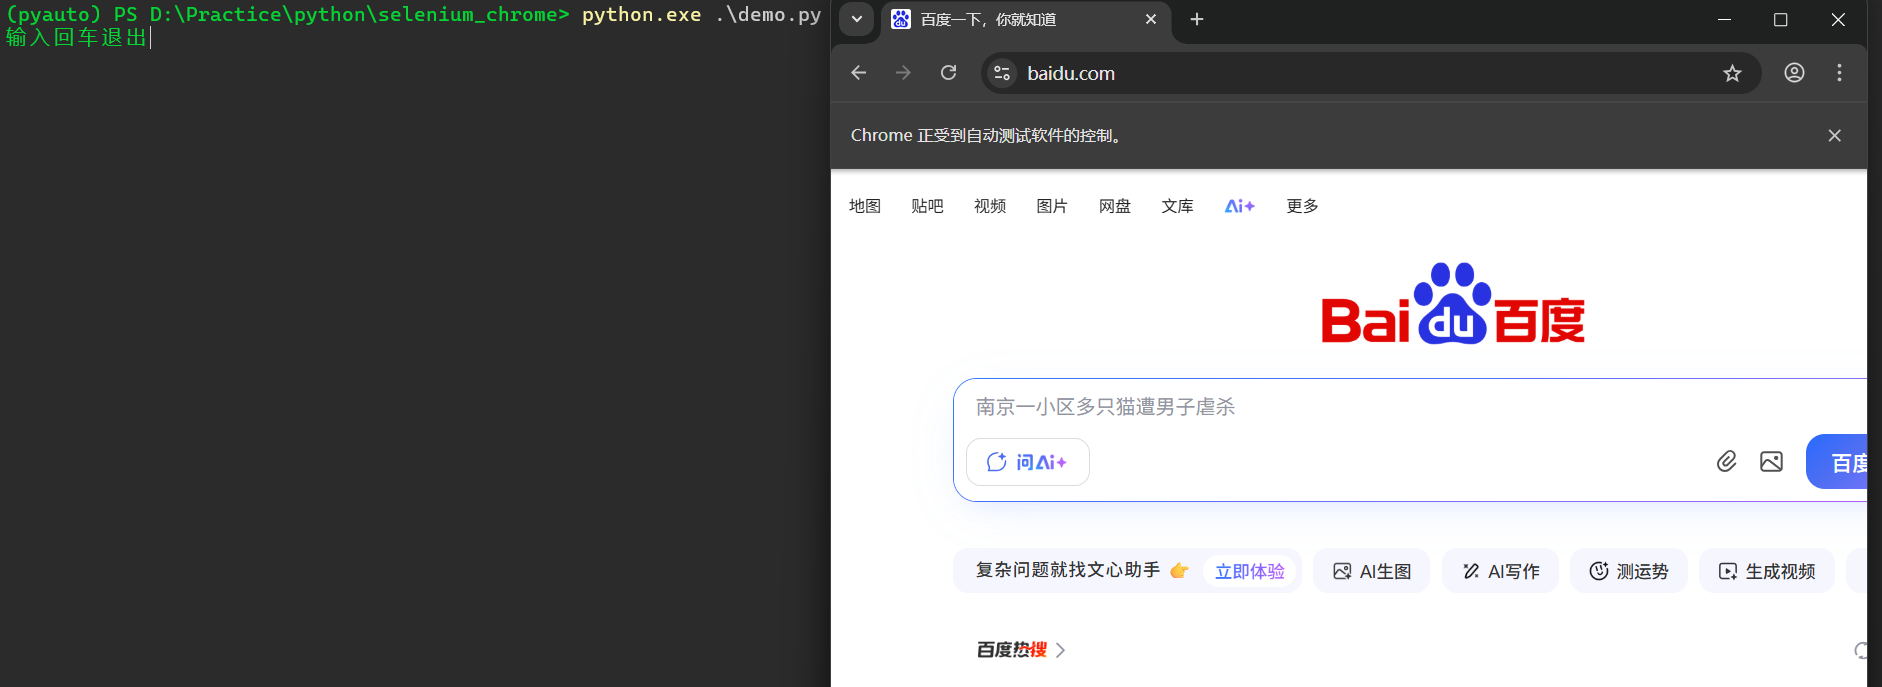
\includegraphics[width=0.6\textwidth]{part/自动化/网页自动化/pic/Selenium/概述/自动下载相应的驱动.png}
    \caption{Selenium4.0以后自动下载相应的驱动}
\end{figure}

\textcolor{red}{\textbf{当国内的网络环境，自动检测下载驱动需要不一样的网络环境，所以建议手动下载驱动，然后指定驱动路径。}}

\begin{lstlisting}[style=demostyle,numbers=none]
from selenium import webdriver
from selenium.webdriver.chrome.service import Service
# 在 Selenium 4 中，不再直接在 webdriver.Chrome 中设置驱动程序路径，而是通过引入 Service 对象来设置。
# 这样可以避免弃用警告，并确保驱动程序的正确加载。

service = Service("D:/Practice/python/selenium_chrome/chromedriver.exe") # ChromeDriver路径
browser = webdriver.Chrome(service=service)     # 创建浏览器对象

# 访问网址
browser.get(f"https://www.baidu.com/")  

# 定位元素

# 保持浏览器不退出
s = input("输入回车退出")
\end{lstlisting}
\begin{figure}[htpb]
    \centering
    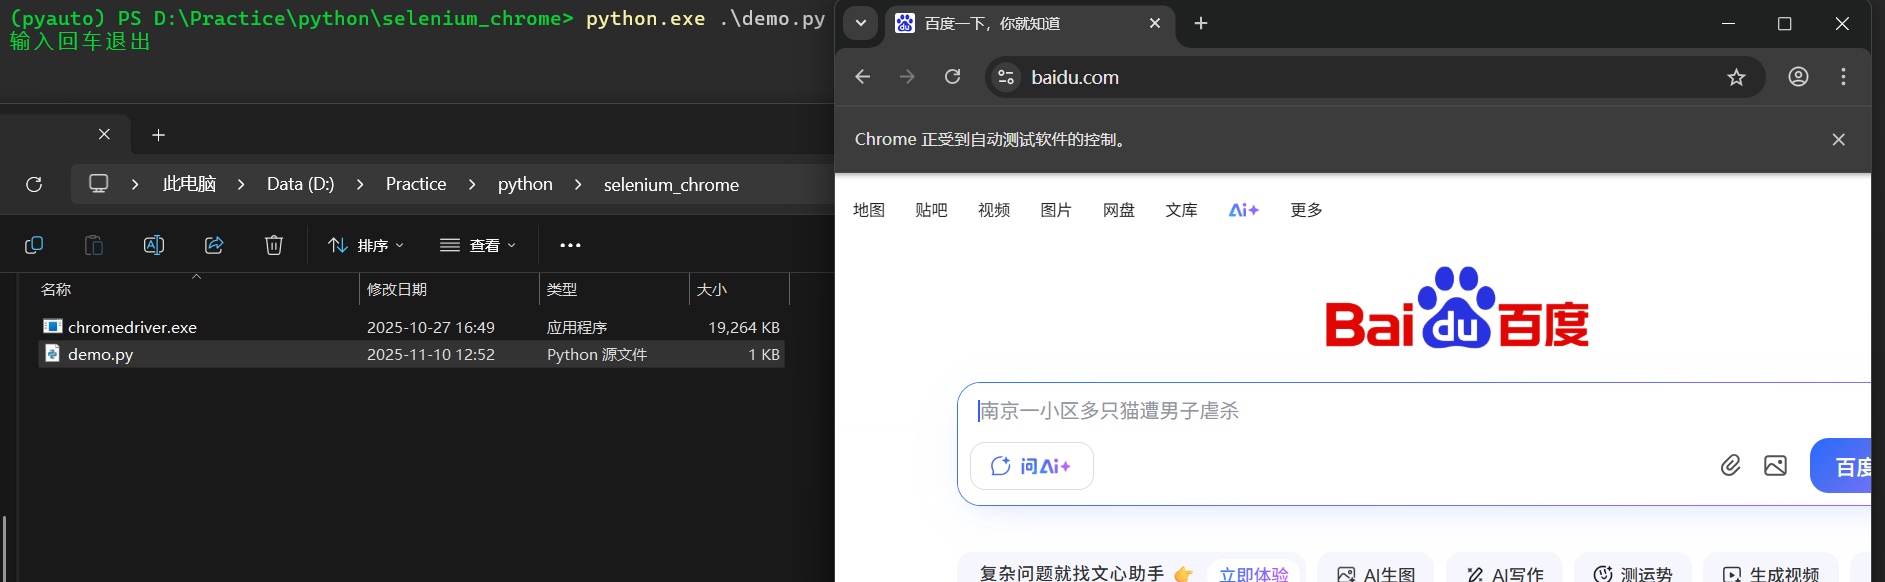
\includegraphics[width=0.6\textwidth]{part/自动化/网页自动化/pic/Selenium/概述/Selenium4指定驱动位置.png}
    \caption{Selenium4指定驱动位置}
\end{figure}
\end{enumerate}

\subsection{Selenium 操作流程}
\begin{lstlisting}[style=demostyle,numbers=none]
from selenium import webdriver
from selenium.webdriver.chrome.service import Service as ChromeService    

# 1.设置正确的驱动路径
service = ChromeService(executable_path="D:/Practice/python/selenium_chrome/chromedriver.exe")

# 2.[可选] 设置开机启动参数
options = webdriver.ChromeOptions() # 创建ChromeOptions对象
options.add_argument("--start-maximized") # 窗口最大化

# 3.创建浏览器对象
browser = webdriver.Chrome(service=service, options=options)

# 4.访问网址
browser.get(f"https://www.baidu.com/")

# 5.定位元素

# 6.操作元素

# 7.[可选] 保持浏览器不退出

# 7.[可选] 操作完成后关闭浏览器
browser.quit()
\end{lstlisting}


